
% \begin{itemize}
%     \item What is OCR 
%     \item Datasets (types(synthetic, photos, scaned documents),problems(languages, noise, nonhorizontal text))
%     \item Text detection
%     \begin{itemize}
%         \item Description
%         \item Methods (CRAFT)
%     \end{itemize}
%     \item Text recognition
%     \begin{itemize}
%         \item Description
%         \item Methods 
%     \end{itemize}
%     \item End-to-end systems (Annotating tool)
%     \begin{itemize}
%         \item[] Reading scanned documents
%         \item EasyOCR
%         \item keras-ocr
%         \item Tesseract (PyTesseract)
%         \item (Google Cloud Vision free) paid
%         \item (AWS Recognition) paid 
%         \item (Kili) paid
%     \end{itemize}
%     \item Results evaluation
%     \begin{itemize}
%         \item Comparison of output and ground-truth
%         \item Bag of words
%     \end{itemize}
%     \item Testing methods on free datasets
%     \item[] Description of datasets
%     \item Using methods on historical posters    
%     \item[] Description of dataset

\chapter{OCR tools}
\label{ch:sw}
OCR software can be divided in four main types by its functionality - text detector, text recognizer and full OCR engine. The last one can either be an end-to-end system, which does both detection and recognition together which means that these two processes influence each other, or a tool that combines a separate detector and recognizer. For an end user who needs to convert text from an image into a computer readable format. The supply of such tools is wide, ranging from open source libraries for various programming languages to commercial softwares with modern GUI. New methods are still being developed as there is always space for improvement. New methods can come from commercial background or are developed for international OCR competitions. In the next sections a selection of the free available tools is described.

\section{CRAFT}

Character Region Awareness for Text Detection (CRAFT) is framework for scene text detection introduced by Clova AI research group. It uses a Convolutional Neural Network. It performs well also on curved or differently deformed texts. Its methodology is to localize individual characters then characters belonging to the same word (based on distance) can be connected into word box or polygon. After that bounding box is created around it and output contains the rectangle coordinates.\cite{craft2}

CRAFT uses  a fully convolutional neural network based on VGG-16.%najit vgg16 a popsat!!!
The network returns two values -- an affinity and region score. "The region score represents the probability that the given pixel is the center of the character and the affinity score represents the center probability of the space between adjacent characters" \cite[page 3]{craft2}. Because CRAFT detect individual characters it was necessary for the authors to create ground truth with bounding boxes for each character. Both scores, thus the probabilities they represent, are encoded with a Gaussian heatmap which is often used were ground truth regions are not strictly bounded. The model was trained on a synthetic dataset SynthText for 50k iterations, further weakly-supervised training was performed on ICDAR datasets.\cite{craft2}

This method has similarly successful performance as other state-of-the-art methods and in last years it is often used as a detection tool in systems that recognize text from unsegmented images. There exists an official Pytorch implementation of CRAFT for python which can be cloned from Clova AI GitHub repository\footnote{https://github.com/clovaai/CRAFT-pytorch}, however it is not a python package. A package for python of CRAFT detector exists under the name \texttt{
craft-text-detector}.

\section{Tesseract}

Tesseract is an open source text recognition engine. It supports over 160 languages can be trained to recognize new ones. Originally Tesseract was created by Hewlett-Packard in late 1980s, from 2006 it is developed and maintained by Google. As it does not have a built-in GUI direct use is via command line. However, there exist a significant number of GUIs for Linux, Windows, Mac for computer usage and also for Android and iOS to use on mobile phones and few online OCR services. Another way how to use the engine is via libraries for computer languages, namely for example they exist for Java called tess4j, python called pytesseract, R, Ruby and others. \cite{tesseract1}

Tesseract is mainly used as tool for recognizing documents (with both computer font text or hadwritten text). Best results are obtained on preprocessed images. The preprocessing includes noise reduction, horizontal alignment of text, elimination of dark borders around text region, conversion to binary black and white picture and other adjustments depending on the nature of the picture. The ideal image for Tesseract is a legible, typed, black text on plain white. Thus when used on scene text images it gives generally worse results than other OCR softwares. 

Computations with Tesseract are supported for GPU and also CPU. Since version 4, that was announced in 2018, Tesseract uses for recognition Long Short Term Memory (LSTM) model (kind of RNN). A simple pipeline of Tesseract is in Figure \ref*{img:tesseractPipeline}. First a binary image is created from the input one, then characters are found with the connected components algorithm. Joined characters are then chopped and broken ones are connected, now each character should be separate. Then characters are recognized and further joined into words. The words are verified in a lexicon and a word with the smallest distance is selected.\cite{tesseract2}

\begin{figure}[hbtp]
    \centering
    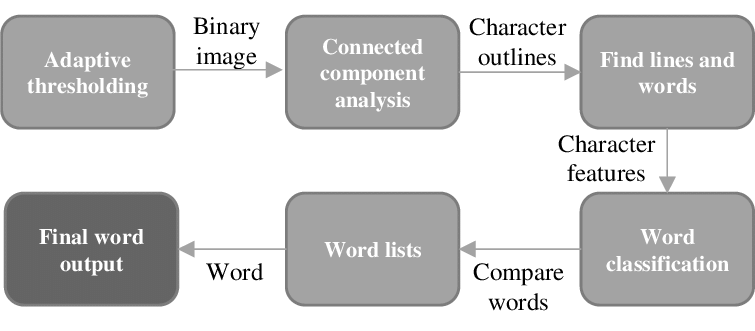
\includegraphics[scale=0.4]{obrazky/tesseract.png}
    \caption{Pipeline architecture of Tesseract OCR engine. \cite{tessPipeline}}
    \label{img:tesseractPipeline}
\end{figure}


By default Tesseract expects a page of text -- black letters on white background grouped in horizontal lines, where font type and font size vary only slightly. To deal with differently distributed text over an image Tesseract provides thirteen page segmentation models (PSM). When selecting the right model Tesseract performance can increase from zero up to almost perfect results. Description of all the PSMs can be find directly via Tesseract help command in console application. Thanks to the various PSM Tesseract works also as a detection tool but often happens that during a search for text in scene images it mistakes objects and structers for text. Such example can be seen in Figure \ref*{img:tesseractMiss}. Besides the PSM parameter user can set also OCR engine modes (OEM). There are four settings differing in whether a LSTM network should be used. 

\begin{figure}[hbtp]
    \centering
    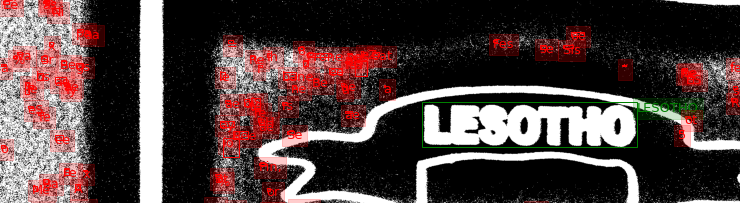
\includegraphics[scale=0.55]{obrazky/result_tesseract_CTW_u_miss.png}
    \caption{Tesseract mistakes background texture for text. Red rectangles and characters denotes predicted words. Part of an preprocessed image from CTW1500 dataset.}
    \label{img:tesseractMiss}
\end{figure}


\section{EasyOCR}

EasyOCR is a product of Jaded AI for both image text detection and recognition. it supports over 80 languages and various scripts such as Latin, Chinese, Arabic etc. The company offers software with web interface for free and also prepaid version which enables usage of a new model for custom data. However, in addition to the web interface, the company also created a python package under the same name.\cite{easyocr1}

The product is still in development and aims for wider functionality. A future idea of EasyOCR package is to provide an easy-to-use tool where one can plug-in already created state-of-the-art models and use them for annotating. Pipeline of EasyOCR behavior is shown in the image \ref*{img:easyocrPipeline}. As it can be seen in this image, default detection model is CRAFT and for recognition is used CRNN (Convolutional Recurrent Neural Network)\footnote{The description of this network is in Chapter \ref*{sec:CRNN}.}. The implementation of this network is composed of following components: feature extraction (Resnet is used) and VGG (Convolutional Neural Network), sequence labeling (BLSTM is used) and decoding (CTC is used).\cite{easyocr2}

EasyOCR package by default computes annotation on GPU, however there is a possibility for CPU computations (provided that the selected model supports it). 

\begin{figure}[hbtp]
    \centering
    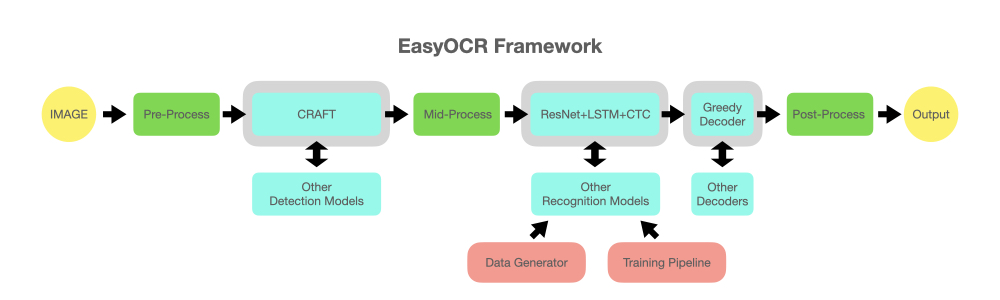
\includegraphics[scale=0.4]{obrazky/easyocr_framework.jpeg}
    \caption{Diagram of EasyOCR pipeline. Grey slots are placeholders for models. The mentioned models are the ones used as default. \cite{easyocr2}}
    \label{img:easyocrPipeline}
\end{figure}

\section{Keras-ocr}

keras-ocr is a python library used for detecting and recognizing text in images created by Fausto Morales. It works with variety of languages and with different writing scripts. It allows computing on CPU as well as on GPU.  It unites the CRAFT text detection model and an implementation in Keras python library of CRNN for recognizing text, worth mentioning this is a different implementation of CRNN than in EasyOCR.\cite{keras-ocr1}

On the official website\footnote{\url{https://pypi.org/project/keras-ocr/}} of the package there is a comparison of this method with two other OCR APIs -- Google Cloud Vision and AWS Rekognition. Their performance was tested on 1,000 images from the COCO-Text validation set using a basic pretrained model of each method. None of the investigated methods performed poorly; however, AWS Rekognition had the worst precision and recall results. Google's method and keras-ocr has similar results. It is important to mention that no tuning parameters were used in any of these methods. Another candidate for comparison was Tesseract but it performed on very badly on given data, most likely due to the fact that Tesseract is suitable for scanned documents rather than for photos of real life scenery and objects with text. \cite{keras-ocr1}

CRAFT already provides a pretrained model which can be used directly without modification for text detection or it is used as initial model for training a new model on new data. This model was trained on three datasets (SynthText, IC13, IC17) and supports English and multi language text detection.\cite{craft1}
Similarly for recognition, CRNN also has a pretrained model. This model was trained on the synthetic word dataset which consists of 9 million images with vocabulary of 90K English words.\cite{synth}
To use these models in the keras-ocr library one either doesn't specify anything and use the defaults, or pass the value \texttt{clovaai-general} for the CRAFT pretrained model or \texttt{kurapan} for the CRNN model.

Keras-ocr offers preprocessing for four public datasets though any text image dataset can be examined using this tool. These four datasets are: BornDigital dataset, COCO-Text dataset, ICDAR 2013 dataset, ICDAR 2019 dataset (only Latin-only scripts).\cite{keras-ocrDocu}


% \section{Other}

% % \subsubsection{AWS Rekognition}

% \subsection*{Google Cloud Vision}

% Google Cloud Vision is software from Google which consist of two products: AutoML Vision and Vision API. Vision API detects objects, faces and text from images with already pretrained model. With AutoML Vision user can train custom model from own data. It has free and paid version with a GUI.\cite{google1}
% % @misc{google1, title={Vision AI | derive image insights via ML &nbsp;|&nbsp; cloud vision API &nbsp;|&nbsp; google cloud}, url={https://cloud.google.com/vision/}, journal={Google}, publisher={Google}} 
% % API for python
